\documentclass[14pt]{extarticle}

\usepackage{fontspec}
\setmainfont{Times New Roman}

% размер полей
\usepackage{geometry}
\geometry{a4paper, top=2cm, bottom=2cm, right=1.5cm, left=3cm}

 %debugging
%\usepackage{showframe}

% полуторный интервал
\usepackage{setspace}
\onehalfspacing

% абзацный отступ
\setlength{\parindent}{1.25cm}

% выравнивание текста по ширине
\sloppy

% списки
\usepackage{calc} % арифметические операции с величинами
\usepackage{enumitem}
\setlist{
    nosep,
    leftmargin=0pt,
    itemindent=\parindent + \labelwidth - \labelsep,
}

% подписи к рисункам и таблицам
\usepackage{caption}
\renewcommand{\figurename}{Рисунок}
\renewcommand{\tablename}{Таблица}
\DeclareCaptionFormat{custom}
{
    \textit{#1#2#3}
}
\DeclareCaptionLabelSeparator{custom}{. }
\captionsetup{
    % хз какой это размер - 12 или нет, но выглядит меньше 14
    font=small,
    format=custom,
    labelsep=custom,
}

% картинки
\usepackage{graphicx}

% колонтитулы
\usepackage{fancyhdr}

% картинки и таблицы находятся именно в том месте текста где помещены (атрибут H)
\usepackage{float}

% таблицы
\usepackage{tabularray}

\graphicspath{ {6.3.5/models/} }
\begin{document}
\pagestyle{fancy}
\fancyhead{}
% disable header
\renewcommand{\headrulewidth}{0pt}
\fancyfoot[L]{Дубровских гр 221-361}
\fancyfoot[C]{ЛР 6.3.5}
\fancyfoot[R]{Продажа автотранспорта}
\singlespacing

\newpage
\begin{center}
    Министерство науки и высшего образования Российской Федерации
    Федеральное государственное автономное образовательное учреждение

    высшего образования

    \guillemotleft МОСКОВСКИЙ ПОЛИТЕХНИЧЕСКИЙ УНИВЕРСИТЕТ\guillemotright

    (МОСКОВСКИЙ ПОЛИТЕХ)
\end{center}
\noindent
\bigbreak
\bigbreak
\bigbreak
\bigbreak
\begin{center}
    ЛАБОРАТОРНАЯ РАБОТА 5.2.1

    По курсу Проектирования пользовательских интерфейсов в веб

    \textbf{Проектирование композиции и визуальной иерархии в макете веб-страниц и мобильного устройства}
    \bigbreak
    \bigbreak
    \bigbreak
    \bigbreak
    ТЕМА

    \guillemotleft\textbf{САЙТ ДЛЯ ПРОДАЖИ И ПОИСКА АВТОМОБИЛЕЙ}\guillemotright
\end{center}
\noindent
\bigbreak
\bigbreak
\bigbreak
\bigbreak
\bigbreak
\bigbreak
\bigbreak
\bigbreak
\bigbreak
\bigbreak
\hfill Выполнил

\hfill Дубровских Никита Евгеньевич

\hfill Группа 221-361
\bigbreak
\bigbreak
\bigbreak
\hfill Проверил

\hfill Натур ВВ
\vfill
\begin{center}
    Москва, 2024
\end{center}
\newpage
\onehalfspacing


\begin{center}
    \textbf{Лабораторная работа 6.3.5}

    \textbf{Оптимизации изображений для веб-контента}
\end{center}

\textbf{Цель работы:} оптимизировать необходимый графический веб-контент пользовательского интерфейса
\bigskip

\textbf{Задачи:}

\begin{enumerate}
    \item В качестве примера проследить (провести) оптимизацию фотографического изображения для сайта строительной компании https://1ps.ru/blog/texts/2016/gotovim-kartinki-dlya-sajta/)
    \item Оптимизировать и обработать 2-3 изображения и графику для веб-страниц по специфике проектного сайта и приложения. Пройти оптимизацию по всем возможным этапам. Оформить результат в Сводную таблицу.
    \item Разместить в вайфреймах подобранные изображения в соответствии с тематикой, стилем и ЦА веб-сайта.
\end{enumerate}
\bigskip

\textbf{Основные термины}

\begin{itemize}
    \item Оптимизация изображений — процесс преобразования изображений в подходящий формат, разрешение и размер для улучшения их загрузки на веб-странице без потери качества. Это включает сжатие файлов, выбор формата, изменение размеров и других параметров, чтобы обеспечить быструю загрузку и улучшить взаимодействие пользователя.
    \item Параметры изображения — основные характеристики изображений, такие как разрешение, «вес» (размер файла), пропорции, качество и формат. Эти параметры влияют на скорость загрузки, восприятие пользователями и SEO.
    \item Сжатие изображения — уменьшение размера файла за счет удаления избыточных данных (с потерями или без потерь) с сохранением высокого визуального качества. Популярные способы сжатия включают использование форматов JPEG, PNG и WebP.
    \item Форматы изображений — JPEG, PNG, GIF, SVG, WebP, AVIF и другие. Каждый формат имеет свои особенности: JPEG подходит для фотографий, PNG для графики с прозрачностью, GIF для анимации, WebP и AVIF для уменьшения размера с высоким качеством.
    \item Памятные цвета — естественные цвета, которые пользователи ожидают видеть на изображениях (телесные тона, зелень, голубое небо и др.). Правильная настройка таких цветов помогает улучшить качество изображения и восприятие пользователями.
    \item Размер файла — объем памяти, который занимает изображение. Он зависит от количества пикселей и сжатия. Малый размер важен для быстрой загрузки сайта.
    \item Миниатюра (превью) — уменьшенное изображение, используемое для списка товаров или статей. Миниатюры ускоряют загрузку сайта, уменьшая нагрузку на сервер.
    \item Атрибут alt — текстовое описание изображения, которое вставляется в код HTML. Он помогает поисковым системам индексировать изображение и полезен для доступности, отображая текст при невозможности загрузки изображения.
    \item Пропорции изображения — соотношение сторон изображения (например, 4:3, 16:9, 1:1), которые влияют на его размещение на веб-странице и восприятие пользователями.
    \item Уникальность изображения — параметр, отражающий оригинальность графического контента. Проверка уникальности важна для SEO и предотвращения копирования.
\end{itemize}
\bigskip

\textbf{Оптимизация образца примера}
\bigskip

Исходное изображение:

\noindent
\begin{minipage}{\linewidth}
    \fbox{\includegraphics[width=\linewidth]{source}}
    \captionof{figure}{Исходное изображение}
\end{minipage}
\bigskip

Уменьшим ширину до 1024 пикселей, сохраняя пропорции.

\noindent
\begin{minipage}{\linewidth}
    \fbox{\includegraphics[width=\linewidth]{source_resolution_gimp}}
    \captionof{figure}{Gimp уменьшение ширины}
\end{minipage}
\bigskip

\noindent
\begin{minipage}{\linewidth}
    \fbox{\includegraphics[width=\linewidth]{source_scaled}}
    \captionof{figure}{Gimp уменьшенное}
\end{minipage}
\bigskip

Обрежем лишнее.

\noindent
\begin{minipage}{\linewidth}
    \fbox{\includegraphics[width=\linewidth]{source_cropped}}
\end{minipage}
\bigskip

Увеличим яроксть и контраст

\noindent
\begin{minipage}{\linewidth}
    \fbox{\includegraphics[width=\linewidth]{source_brightness_contrast}}
\end{minipage}
\bigskip

Сделаем фотографию более "теплой"

\noindent
\begin{minipage}{\linewidth}
    \fbox{\includegraphics[width=\linewidth]{source_temperature}}
\end{minipage}
\bigskip

Сохраним в оптимальном для вебa качестве 75\%

\noindent
\begin{minipage}{\linewidth}
    \fbox{\includegraphics[width=\linewidth]{source_quality}}
\end{minipage}
\bigskip

Сжимаем картинку в сервисе "tinypng.com"

\noindent
\begin{minipage}{\linewidth}
    \fbox{\includegraphics[width=\linewidth]{tinypng}}
\end{minipage}
\bigskip

\noindent
\begin{minipage}{\linewidth}
    \fbox{\includegraphics[width=\linewidth]{source_tinypng}}
\end{minipage}
\bigskip

Создадим превью

\noindent
\begin{minipage}{\linewidth}
    \fbox{\includegraphics{source_preview}}
\end{minipage}
\bigskip

Итог
\bigskip

\begin{table}[H]
\centering
\begin{tblr}{
  hlines,
  vlines,
}
Изображение      & Разрешение & Вес      \\
Оригинал         & 1944x2592  & 2,2 Мб   \\
Оптимизированное & 836x882    & 126,3 Кб \\
Превью           & 300x317    & 19,6 Кб  
\end{tblr}
\end{table}

\textbf{Оптимизация изображений для веб-страниц}

\noindent
\begin{minipage}{\linewidth}
    \fbox{\includegraphics[width=\linewidth]{nature}}
    \captionof{figure}{Исходное изображение}
\end{minipage}
\bigskip

\noindent
\begin{minipage}{\linewidth}
    \fbox{\includegraphics[width=\linewidth]{nature_cropped}}
    \captionof{figure}{Обрезанное}
\end{minipage}
\bigskip

\noindent
\begin{minipage}{\linewidth}
    \fbox{\includegraphics[width=\linewidth]{gimp_scale_nature}}
    \captionof{figure}{Разрешение}
\end{minipage}
\bigskip

\noindent
\begin{minipage}{\linewidth}
    \fbox{\includegraphics[width=\linewidth]{nature_cropped_scaled}}
    \captionof{figure}{Уменьшенное}
\end{minipage}
\bigskip

\noindent
\begin{minipage}{\linewidth}
    \fbox{\includegraphics{gimp_scale_quality_nature}}
    \captionof{figure}{Качество}
\end{minipage}
\bigskip

\noindent
\begin{minipage}{\linewidth}
    \fbox{\includegraphics[width=\linewidth]{nature_cropped_scaled_quality}}
    \captionof{figure}{75\% качество}
\end{minipage}
\bigskip

\noindent
\begin{minipage}{\linewidth}
    \fbox{\includegraphics[width=\linewidth]{nature_tinypng}}
    \captionof{figure}{Оптимизация через tinypng}
\end{minipage}
\bigskip

\noindent
\begin{minipage}{\linewidth}
    \fbox{\includegraphics[width=\linewidth]{nature_cropped_scaled_quality_tinypng}}
    \captionof{figure}{После оптимизация через tinypng}
\end{minipage}
\bigskip

\noindent
\begin{minipage}{\linewidth}
    \fbox{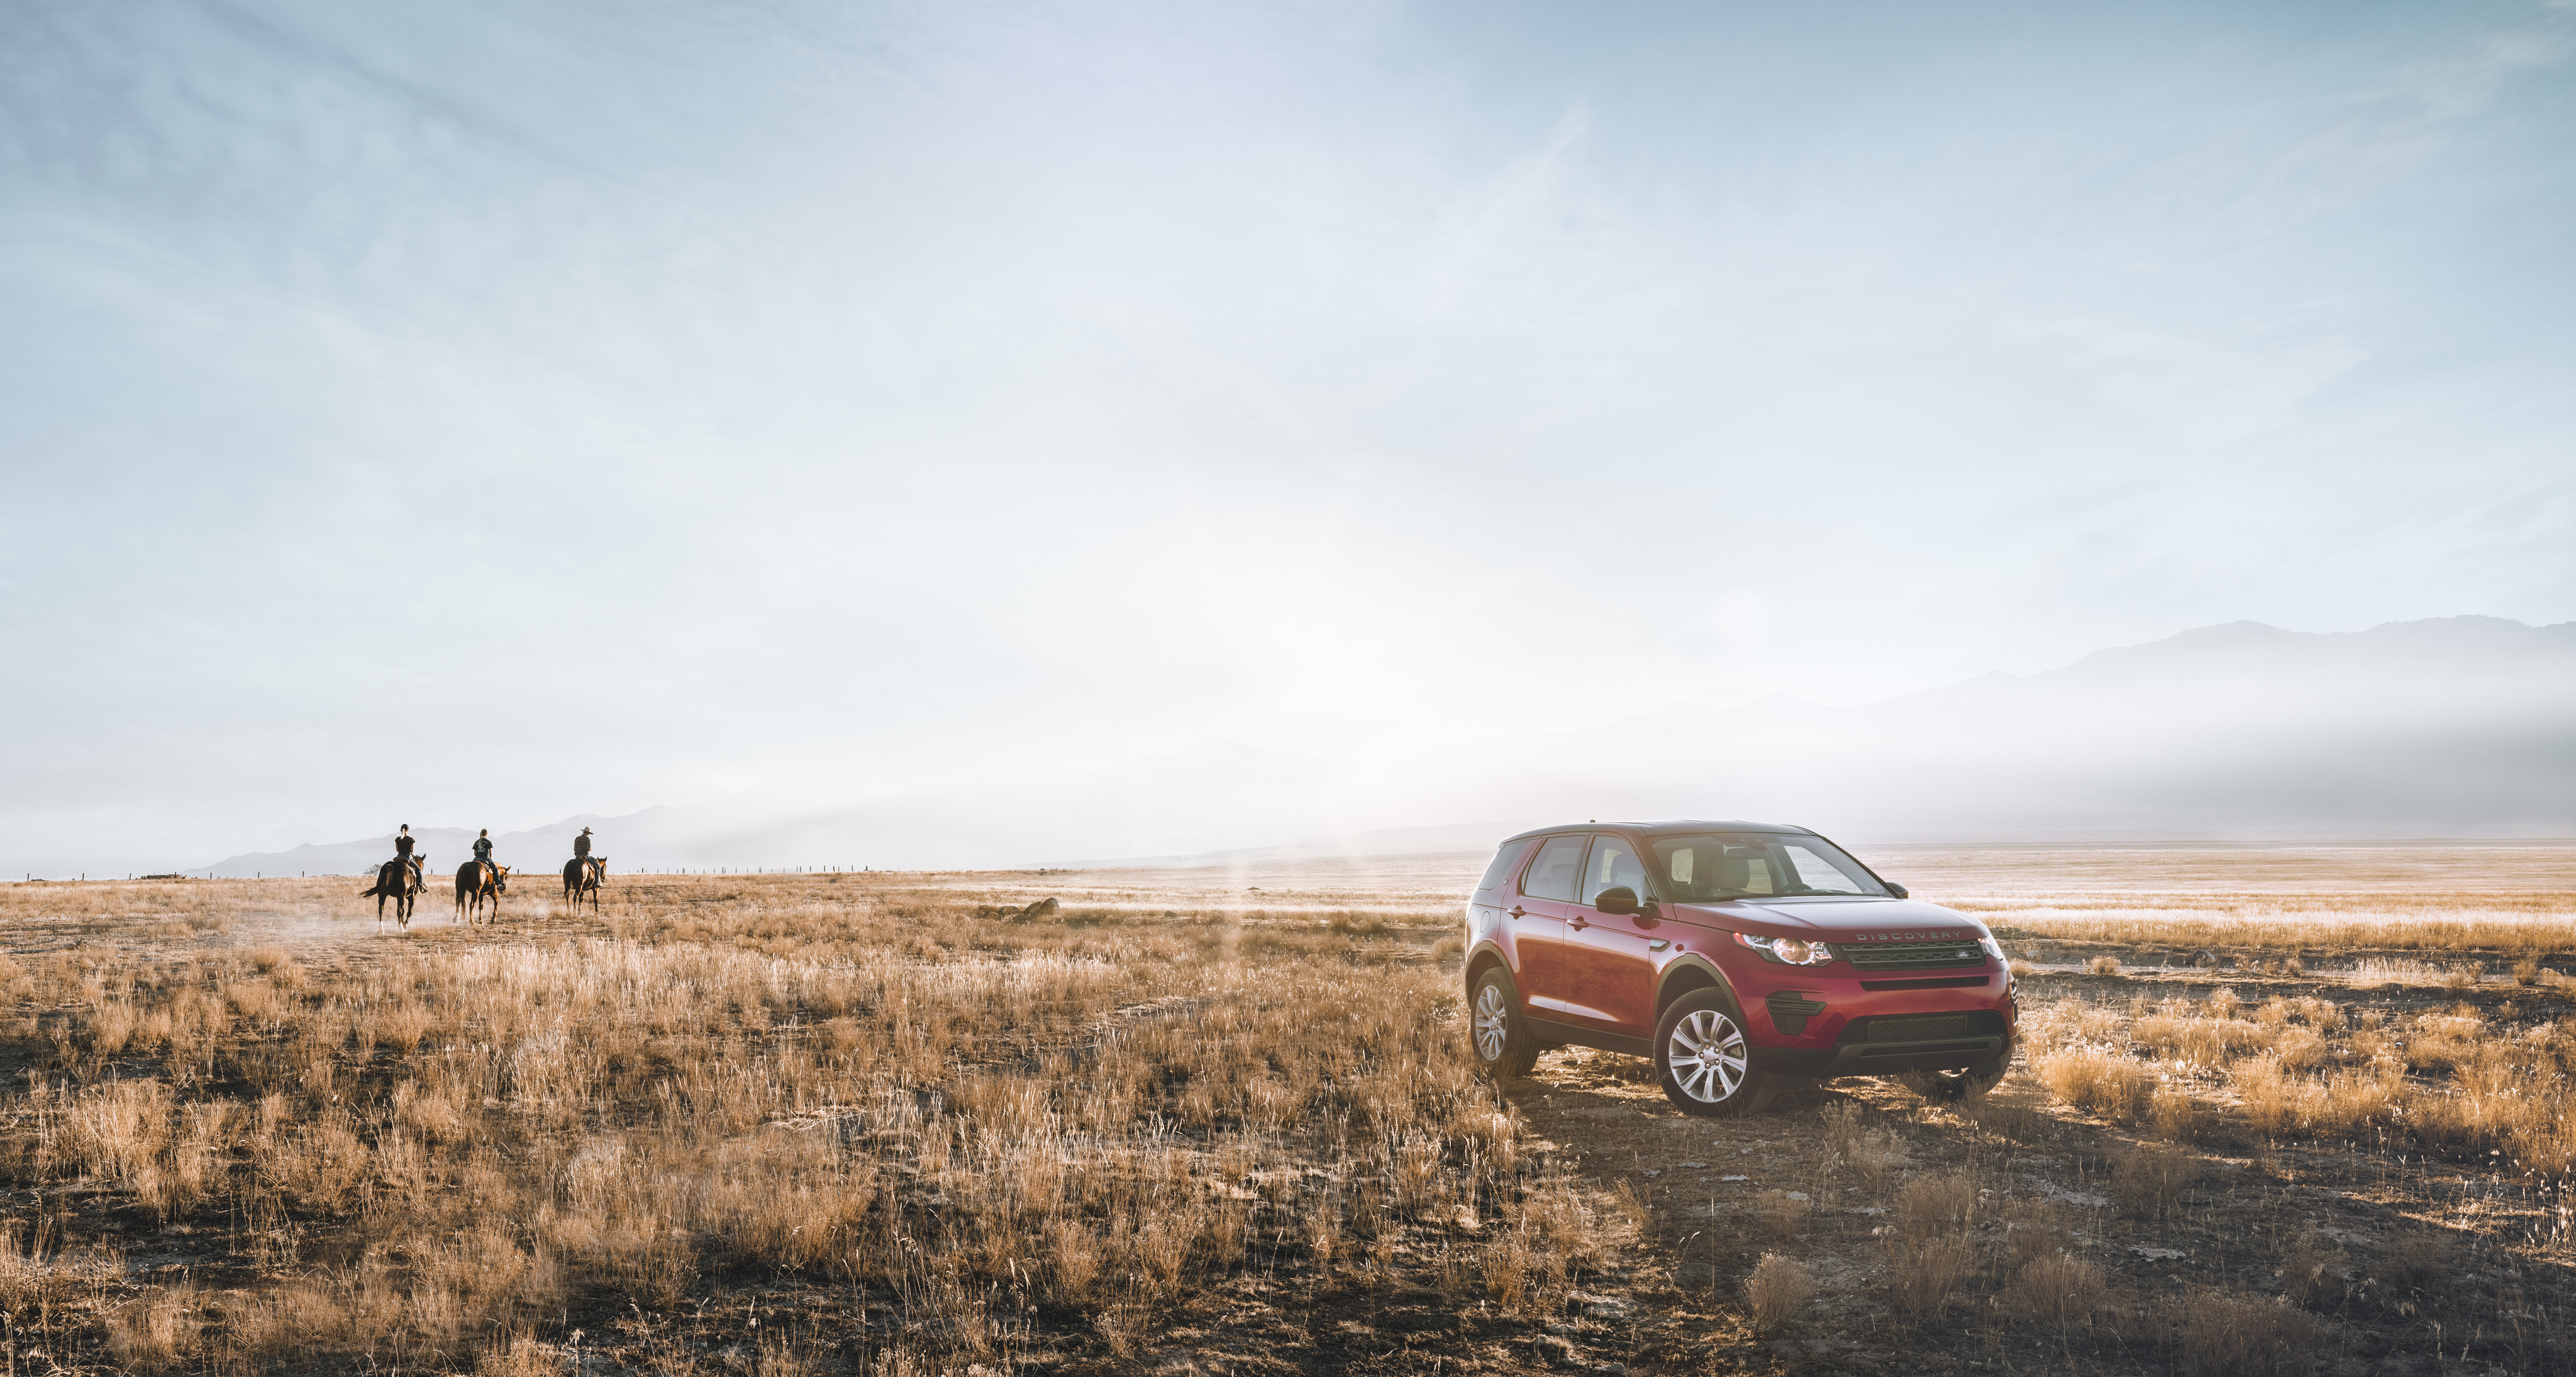
\includegraphics[width=\linewidth]{step_mashina_loshadi}}
    \captionof{figure}{Исходное изображение}
\end{minipage}
\bigskip

\noindent
\begin{minipage}{\linewidth}
    \fbox{\includegraphics[width=\linewidth]{step_cropped}}
    \captionof{figure}{Обрезанное}
\end{minipage}
\bigskip

\noindent
\begin{minipage}{\linewidth}
    \fbox{\includegraphics[width=\linewidth]{gimp_step_scale}}
    \captionof{figure}{Разрешение}
\end{minipage}
\bigskip

\noindent
\begin{minipage}{\linewidth}
    \fbox{\includegraphics[width=\linewidth]{step_scaled}}
    \captionof{figure}{Уменьшенное}
\end{minipage}
\bigskip

\noindent
\begin{minipage}{\linewidth}
    \fbox{\includegraphics{gimp_scale_quality_nature}}
    \captionof{figure}{Качество}
\end{minipage}
\bigskip

\noindent
\begin{minipage}{\linewidth}
    \fbox{\includegraphics[width=\linewidth]{step_quality}}
    \captionof{figure}{75\% качество}
\end{minipage}
\bigskip

\noindent
\begin{minipage}{\linewidth}
    \fbox{\includegraphics[width=\linewidth]{step_tinypng}}
    \captionof{figure}{Оптимизация через tinypng}
\end{minipage}
\bigskip

\noindent
\begin{minipage}{\linewidth}
    \fbox{\includegraphics[width=\linewidth]{step_tinypng_image}}
    \captionof{figure}{После оптимизация через tinypng}
\end{minipage}
\bigskip

\noindent
\begin{minipage}{\linewidth}
    \includegraphics[width=\linewidth]{tables}
\end{minipage}
\bigskip

\textbf{Контрольные вопросы и ответы}

\begin{enumerate}
    \item Какую роль играют параметры изображений для веб?

    Параметры изображений, такие как разрешение, размер файла, качество и формат, напрямую влияют на скорость загрузки веб-страницы, её эстетическую привлекательность и восприятие пользователем. Оптимизация этих параметров обеспечивает хорошее качество изображения при минимальном размере файла, что способствует более быстрому загрузке и улучшенному пользовательскому опыту.

    \item Что такое оптимизация изображений?

        Оптимизация изображений — это процесс преобразования изображений в нужный формат, размер и разрешение для веб-среды с целью уменьшения их «веса» и улучшения качества отображения. Это включает сжатие, изменение разрешения и улучшение параметров изображения для минимизации времени загрузки сайта и повышения его производительности.

    \item Какие существуют рекомендации разрешению и «весу» изображений для веб-интерфейса?

    Максимальная ширина изображения не должна превышать 1024 пикселей.
    Вес файла должен быть не больше 80–100 килобайт для стандартных изображений и не более 250 килобайт для больших изображений.
    Использовать подходящие форматы (JPEG, PNG, WebP) и сжатие для уменьшения размера без потери качества.

    \item Как оптимизируются изображения по памятным цветам?

        Оптимизация по памятным цветам включает в себя улучшение естественных оттенков, таких как телесные тона, естественный зеленый, голубое небо и другие цвета, которые легко запоминаются и важны для восприятия. Это помогает сделать изображение более реалистичным и приятным для восприятия, убирая паразитные оттенки, которые могут возникнуть при неверных настройках.

    \item Какие существуют приёмы по оптимизации изображений для веб-интерфейса?

    Сжатие изображений с помощью сервисов (например, TinyPNG, Optimizilla) или программ (Photoshop, ImageOptim).
    Изменение размеров изображений в пикселях до требуемого разрешения.
    Выбор оптимального формата: JPEG или WebP для фотографий, PNG или SVG для графики.
    Использование правильных пропорций и единообразных размеров на одной странице.
    Установка атрибута alt в тегах изображений для улучшения SEO.
\end{enumerate}

\end{document}
